\documentclass{article}
\usepackage{tikz}
\usetikzlibrary{arrows}
\begin{document}
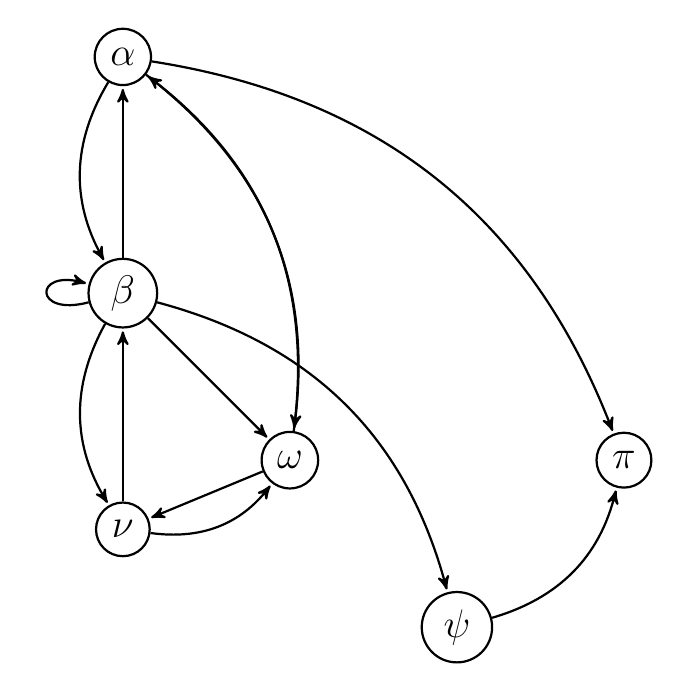
\begin{tikzpicture}[->,>=stealth',shorten >=1pt,auto,node distance=3cm,
  thick,main node/.style={circle,fill=white,draw,font=\sffamily\Large\bfseries}]

  \node[main node] (1) {$\alpha$};
  \node[main node] (2) [below of=1] {$\beta$};
  \node[main node] (3) [below of=2] {$\nu$};
  \node[main node] (4) [below right of=2] {$\omega$};
  \node[main node] (5) [below right of=4] {$\psi$};
  \node[main node] (6) [above right of=5] {$\pi$};

%sintaxis para relaciones
%edge para relaciones
%[bend lado] para hacer un arco

  \path[every node/.style={font=\sffamily\small}]
   (1) edge [bend left] node [left] {} (4)
       edge [bend right] node[left] {} (2)
       edge [bend left] node[left] {} (6)
   (2) edge node [right] {} (1)
       edge node {} (4)
       edge [loop left] node {} (2)
       edge [bend left] node {} (5)
       edge [bend right] node[left] {} (3)
   (3) edge node [right] {} (2)
       edge [bend right] node[right] {} (4)
   (4) edge node [left] {} (3)
       edge [bend right] node [right] {} (1)
   (5) edge [bend right] node [left] {} (6);

\end{tikzpicture}
\end{document}
